%!TEX output_directory = temp
\documentclass[letterpaper, 12pt]{amsart}
	%%%%%%%%%%%%%%%%%%%%%%%%%%%%%%%%%%%%%%%%%%%%%%%%%%%%%%%%%%%%%%%%%%%%%%%%%%%%%%
	%%%%%%%%%%%%%%%%%%%%%%%%%%%% boilerplate packages %%%%%%%%%%%%%%%%%%%%%%%%%%%%
	\usepackage{amsmath,amssymb,amsthm}
	\usepackage[mathscr]{euscript}
	\usepackage{enumerate}
	\usepackage{graphicx}
	\usepackage{mathrsfs}
	\usepackage{color}
	\usepackage{hyperref}
	\usepackage{verbatim}
	\usepackage{stmaryrd}
	\usepackage[margin=1.25in]{geometry}

	\raggedbottom

	%%%%%%%%%%%%%%%%%%%%%%%%%%%%%%%%%%%%%%%%%%%%%%%%%%%%%%%%%%%%%%%%%%%%%%%%%%%%%%
	%%%%%%%%%%%%%%%%%%%%%%%%%%%%% rename the abstract %%%%%%%%%%%%%%%%%%%%%%%%%%%%
	% \renewcommand{\abstractname}{Introduction}

	%%%%%%%%%%%%%%%%%%%%%%%%%%%%%%%%%%%%%%%%%%%%%%%%%%%%%%%%%%%%%%%%%%%%%%%%%%%%%%
	%%%%%%%%%%%%%%%%%%%%%%%%%%%%%%%%%%%%% sets %%%%%%%%%%%%%%%%%%%%%%%%%%%%%%%%%%%
		%% sets 
		\DeclareMathOperator{\N}{\mathbb{N}}
		\DeclareMathOperator{\Z}{\mathbb{Z}}
		\DeclareMathOperator{\Zp}{\mathbb{Z}^{+}}
		\DeclareMathOperator{\Q}{\mathbb{Q}}
		\DeclareMathOperator{\Qp}{\mathbb{Q}^{+}}
		\DeclareMathOperator{\Qc}{\mathbb{Q}^{c}}
		\DeclareMathOperator{\R}{\mathbb{R}}
		\DeclareMathOperator{\F}{\mathbb{F}}
		\DeclareMathOperator{\Rp}{\mathbb{R}^{+}}
		\DeclareMathOperator{\C}{\mathbb{C}}
		\DeclareMathOperator{\Cnon}{\mathbb{C}^{\times}}
		%% powerset of a set
		\DeclareMathOperator{\pset}{\mathcal{P}}
		%% set of continuous functions in a certain variable
		\DeclareMathOperator{\cont}{\mathscr{C}}
		%% set of functions in a certain variable
		\DeclareMathOperator{\func}{\mathscr{F}}
		
	%%%%%%%%%%%%%%%%%%%%%%%%%%%%%%%%%%%%%%%%%%%%%%%%%%%%%%%%%%%%%%%%%%%%%%%%%%%%%%
	%%%%%%%%%%%%%%%%%%%%%%%%%%%%%%%% linear algebra %%%%%%%%%%%%%%%%%%%%%%%%%%%%%%
		%% linear span
		\DeclareMathOperator{\Ell}{\mathscr{L}}
		%% bold vectors with arrows, and bold matrices
		\newcommand{\bmat}[1]{{\mathbf{#1}}}
		\newcommand{\bvec}[1]{{\vec{\mathbf{#1}}}}
		%% independent vectors/matrices
		\DeclareMathOperator{\ind}{\perp\!\!\!\perp}
		%% order
		\DeclareMathOperator{\ord}{\text{ord}}

	%%%%%%%%%%%%%%%%%%%%%%%%%%%%%%%%%%%%%%%%%%%%%%%%%%%%%%%%%%%%%%%%%%%%%%%%%%%%%%
	%%%%%%%%%%%%%%%%%%%%%%%%%%% probability & statistics %%%%%%%%%%%%%%%%%%%%%%%%%
		%% probability, expectation, variance, etc.
		\renewcommand{\Pr}{\mathbb{P}}
		\DeclareMathOperator{\E}{\mathbb{E}}
		\DeclareMathOperator{\var}{\rm Var}
		\DeclareMathOperator{\sd}{\rm SD}
		\DeclareMathOperator{\cov}{\rm Cov}
		\DeclareMathOperator{\SE}{\rm SE}
		\DeclareMathOperator{\ssreg}{{\rm SS}_{{\rm Reg}}}
		\DeclareMathOperator{\ssr}{{\rm SS}_{{\rm Res}}}
		\DeclareMathOperator{\sst}{{\rm SS}_{{\rm Tot}}}

	%%%%%%%%%%%%%%%%%%%%%%%%%%%%%%%%%%%%%%%%%%%%%%%%%%%%%%%%%%%%%%%%%%%%%%%%%%%%%%
	%%%%%%%%%%%%%%%%%%%%%%%%%%%%%%%% congruences %%%%%%%%%%%%%%%%%%%%%%%%%%%%%%%%%
		\renewcommand{\mod}[1]{\ (\mathrm{mod}\ #1)}

	%%%%%%%%%%%%%%%%%%%%%%%%%%%%%%%%%%%%%%%%%%%%%%%%%%%%%%%%%%%%%%%%%%%%%%%%%%%%%%
	%%%%%%%%%%%%%%%%%%%%%%%%%%%%%% bracket notation %%%%%%%%%%%%%%%%%%%%%%%%%%%%%%
		% I first used this for principal ideals, that is why the abbreviation is pid
		\newcommand{\pid}[1]{\langle #1 \rangle}

	%%%%%%%%%%%%%%%%%%%%%%%%%%%%%%%%%%%%%%%%%%%%%%%%%%%%%%%%%%%%%%%%%%%%%%%%%%%%%%
	%%%%%%%%%%%%%%%%%%%%%%%%%%%%%%% fatdot notation %%%%%%%%%%%%%%%%%%%%%%%%%%%%%%
		\makeatletter
			\newcommand*\fatdot{\mathpalette\fatdot@{.5}}
			\newcommand*\fatdot@[2]{\mathbin{\vcenter{\hbox{\scalebox{#2}{$\m@th#1\bullet$}}}}}
		\makeatother

	%%%%%%%%%%%%%%%%%%%%%%%%%%%%%%%%%%%%%%%%%%%%%%%%%%%%%%%%%%%%%%%%%%%%%%%%%%%%%%
	%%%%%%%%%%%%%%%%%%%%%%%%%%%%%% use pretty letters %%%%%%%%%%%%%%%%%%%%%%%%%%%%
		\DeclareMathOperator{\ep}{\varepsilon}
		\DeclareMathOperator{\ph}{\varphi}

	%%%%%%%%%%%%%%%%%%%%%%%%%%%%%%%%%%%%%%%%%%%%%%%%%%%%%%%%%%%%%%%%%%%%%%%%%%%%%%
	%%%%%%%%%%%%%%%%%%%%%%%%%%% stolen from Jeske/Dugger %%%%%%%%%%%%%%%%%%%%%%%%%
	% Some theorem-like environments, all numbered together starting at 1
	% in each section.

	% The default \theoremstyle is bold headings and italic body text.
	\newtheorem{thm}{Theorem}[section]
	\newtheorem{defn}[thm]{Definition}
	\newtheorem{prop}[thm]{Proposition}
	\newtheorem{claim}[thm]{Claim}
	\newtheorem{cor}[thm]{Corollary}
	\newtheorem{lemma}[thm]{Lemma}

	\theoremstyle{definition}  % Bold headings and Roman body text.
	\newtheorem{example}[thm]{Example}
	\newtheorem{examples}[thm]{Examples}
	\newtheorem{exercise}[thm]{Exercise}
	\newtheorem{note}[thm]{Note}
	\newtheorem{remark}[thm]{Remark}
	\newtheorem{remarks}[thm]{Remarks}
	\newtheorem{discussion}[thm]{Discussion}

	\newcommand{\dfn}{\textbf} % Make defined words bold.
	\newcommand{\mdfn}[1]{\dfn{\mathversion{bold}#1}} % Even make math symbols bold

	% Various commands that are useful.  Please add your own.

	\DeclareMathOperator{\Arg}{Arg}
	\DeclareMathOperator{\re}{Re}
	\DeclareMathOperator{\im}{Im}
	\DeclareMathOperator{\Log}{Log}
	\DeclareMathOperator{\Span}{Span}

	\newcommand{\iso}{\cong}						% isometric/congruent
	\newcommand{\ra}{\rightarrow}                   % right arrow
	\newcommand{\Ra}{\Rightarrow}                   % right implies
	\newcommand{\lra}{\longrightarrow}              % long right arrow
	\newcommand{\la}{\leftarrow}                    % left arrow
	\newcommand{\La}{\Leftarrow}                    % left implies
	\newcommand{\lla}{\longleftarrow}               % long left arrow
	\newcommand{\llra}[1]{\stackrel{#1}{\lra}}      % labeled long right arrow
	\newcommand{\we}{\llra{\sim}}                   % weak equivalence
	\newcommand{\cof}{\rightarrowtail}              % cofibration
	\newcommand{\fib}{\twoheadrightarrow}           % fibration
	\newcommand{\inc}{\hookrightarrow}              % inclusion
	\newcommand{\dbra}{\rightrightarrows}           % double arrow for equalizer diagrams
	\newcommand{\eqra}{\llra{\sim}}                 % equivalence/isomorphism

	% \newcommand{\blank}{\underbar{\ \ }}          % An underscore, as in (__)xV
	\newcommand{\blank}{-}                          % A hyphen, as in (-)xV
	\newcommand{\Id}{Id}                            % The identity functor
	\newcommand{\und}{\underline}
	\newcommand{\norm}[1]{\mid \!\!#1 \!\!\mid}             %\norm{x} gives |x|

	% These commands are for the period and comma in the lower right entry of
	% a diagram.  They put the punctuation 2 pts to the right, but make
	% TeX (and hence the diagram package) unaware of the extra width
	% of that entry.
	\newcommand{\period}    {{\makebox[0pt][l]{\hspace{2pt} .}}}
	\newcommand{\comma}     {{\makebox[0pt][l]{\hspace{2pt} ,}}}
	\newcommand{\semicolon} {{\makebox[0pt][l]{\hspace{2pt} ;}}}

	\newcommand{\Cech}{\v{C}ech}
	\newcommand{\scat}{\Delta}
	\newcommand{\assign}{\ra}
	\newcommand{\copr}{\,\amalg\,}
	\newcommand{\ovcat}{\downarrow}
	\newcommand{\pder}[2]{{\frac{\partial #1}{\partial #2}}}
	\newcommand{\del}{\nabla}
	\newcommand{\vectr}[1]{{\mbox{\boldmath $#1$}}}
	\newcommand{\uvectr}[1]{\vectr{\hat #1}}
	\newcommand{\ihat}{\uvectr \imath}
	\newcommand{\jhat}{\uvectr \jmath}
	\newcommand{\khat}{\uvectr k}
	\newcommand{\rhat}{\uvectr r}
	\newcommand{\thhat}{\uvectr \theta}
	\newcommand{\zhat}{\uvectr z}
	\newcommand{\rhohat}{\uvectr \rho}
	\newcommand{\phihat}{\uvectr \phi}
	\newcommand{\grad}{\vectr{\vec\nabla}}
	% \newcommand{\R}{\mathbb{R}}
	\newcommand{\vv}[1]{\vectr{v_{#1}}}
	\newcommand{\crad}{0.1}
	\newcommand{\lline}[1]{\overleftrightarrow{#1}}
	\DeclareMathOperator{\area}{area}
	\DeclareMathOperator{\vol}{vol}
	\newcommand{\ray}[1]{\overset{\rightarrow}{#1}}
	\newcommand{\sr}[2]{???}
	\newcommand{\iihat}{i}
	\newcommand{\jjhat}{j}
	\newcommand{\kkhat}{k}

	\renewcommand{\abstractname}{Comment}		
\begin{document}
	\title{Homework 3  -- Math 397 \\ \today}
	\author{Alex Thies \\ \href{mailto:athies@uoregon.edu}{\lowercase{athies$@$uoregon.edu}}}

	\maketitle

	\section*{Problem 2}
	Recall that the usual $\sin$ and $\cos$ functions take their inputs in radians. 
	There are different versions of these functions that take their inputs in degrees, which are unfortunately also called ``$\sin$ and $\cos$'' in trigonometry classes—even though they are not the same functions. 
	To clarify things we will write sinD and cosD for the degree-based functions. 
	The functions are related by the formulas
	$$\text{sinD}(x) = \sin \left(\frac{2\pi}{360} x \right), \hspace{5mm} \text{cosD}(x) = \cos \left(\frac{2\pi}{360} x \right).$$

		\subsection*{Part (a)}
		By using the chain rule, show that $\frac{d}{dx}($sinD$) = k \cdot$ cosD $x$ and $\frac{d}{dx}($cosD$) = -k \cdot$ sinD $x$ for a certain constant that you discover.

		\begin{proof}[Solution]
		By the chain rule, we compute the following:
			\begin{align*}
				\frac{d}{dx}\left[ \text{sinD}(x) \right] &= \sin\left( \frac{\pi}{180}x \right), \\
				&= \cos\left( \frac{\pi}{180}x \right)\frac{\pi}{180}, \\
				\\
				\frac{d}{dx}\left[ \text{cosD}(x) \right] &= \cos\left( \frac{\pi}{180}x \right), \\
				&= -\sin\left( \frac{\pi}{180}x \right)\frac{\pi}{180}.
			\end{align*}
		Hence, we have computed the requested derivatives, and have found that $k = \pi/180$, which we recognize as the constant by which we convert angles measured in degrees to radians.
		\end{proof}
		% subsection part_a (end)
		\pagebreak

		\subsection*{Part (b)}
		Recall that $\sin x = x - \frac{x^{3}}{3!} + \frac{x^{5}}{5!} - \cdots$
		Determine the corresponding Taylor series for the sinD function.

		\begin{proof}[Solution]
		We compute the following:
			\begin{align*}
				\sin x &= x - \frac{x^{3}}{3!} + \frac{x^{5}}{5!} - \cdots, \\
				\text{sinD} &= \frac{\pi \cdot x}{180} - \frac{\left( \frac{\pi \cdot x}{180} \right)^{3}}{3!} + \frac{\left( \frac{\pi \cdot x}{180} \right)^{5}}{5!} - \cdots 
			\end{align*}
		Hence, we have the new Taylor series for sinD.
		\end{proof}
		% subsection part_b (end)

		\subsection*{Part (c)}
		Here is a standard calculus problem. 
		A man sits on the ground 1000ft away from the location of a hot air balloon. 
		The balloon starts to rise, and the man measures the angle between the balloon and the ground. 
		When the angle is 30 degrees, he notes that the angle is changing at a rate of 1 degree per minute. 
		What is the vertical velocity of the balloon at this moment?

		The following is a student’s solution:

		Start with $\tan \theta(t) = \frac{h(t)}{1000}$. 
		Differentiate both sides to give $$\sec^{2}( \theta(t)) \cdot \frac{d \theta}{dt} = \frac{1}{1000}\frac{dh}{dt}.$$
		Now plug in $\theta = 30$ and $\frac{d \theta}{dt} = 1$ to get $$\frac{4}{3} \cdot 1 = \frac{1}{1000} \cdot h'(t).$$
		So $h'(t) = 4000/3 \approx 1333.33$, and the units are ft/min. 
		This is the vertical velocity.
		The student’s final answer is totally wrong, although much of the work is correct. 
		Two things for you to do: 
		Explain what is wrong with the student’s solution, and show how to do the problem to obtain the correct answer of $h' = 23.27$ ft/min.

		\begin{proof}[Solution]
		The student is incorrect because they didn't combine the proper units of measure with the proper trigonometric function.
		Notice that the student treats $\tan \theta$ as if $\theta$ is measured in radians, when in fact it is measured in degrees, so when the student computed derivatives, they missed crucial constants that we computed above.
		The appropriate computations are below:
			\begin{align*}
				\frac{d}{dt} \left[ \text{tanD} \ \theta(t) \right] &= \frac{d}{dt} \left[ \frac{h(t)}{1000} \right], \\
				\sec^{2}\left( \frac{\pi}{180}\theta(t) \right) \left( \frac{\pi}{180} \right) \frac{d \theta}{dt} &= \frac{dh}{dt} \frac{1}{1000}, \\
				1000 \left[ \sec^{2}\left( \frac{\pi}{180} \cdot 30 \right) \left( \frac{\pi}{180} \right) 1 \right] &= \frac{dh}{dt}, \\
				\frac{dh}{dt} &= \frac{1000 \pi}{180} \left[ \sec^{2}\left( \pi/6 \right) \right], \\
				&= \frac{1000 \cdot \pi \cdot (4/3)}{180}, \\
				&\approx 23.27^{\circ}.
			\end{align*}
			
		\end{proof}
		% subsection part_c (end)
	% section problem_2 (end)

	\section*{Problem 3}
	There are also hyperbolic sine and cosine functions. 
	They are defined by $$\cosh x = \frac{e^{x} + e^{-x}}{2}, \hspace{5mm} \sinh x = \frac{e^{x} - e^{-x}}{2}.$$

		\subsection*{Part (a)}
		Derive the following identities:
			\subsubsection*{ID - 1}
			\[ \cosh x + \sinh x = e^{x} \]

			\begin{proof}[Solution]
			We compute the following
				\begin{align*}
					\cosh x + \sinh x &= \frac{e^{x} + e^{-x}}{2} + \frac{e^{x} - e^{-x}}{2}, \\
					&= \frac{e^{x} + e^{x} + e^{-x} - e^{-x}}{2}, \\
					&= \frac{2e^{x}}{2}, \\
					&= e^{x}.
				\end{align*}
			Thus, $\cosh x + \sinh x = e^{x}$, as desired.
			\end{proof}
			% subsubsection id_1 (end)
			\pagebreak

			\subsubsection*{ID - 2}
			\[ \frac{d}{dx}(\cosh x) = \sinh x \ \ \text{and} \ \ \frac{d}{dx}(\sinh x) = \cosh x \]

			\begin{proof}[Solution]
			We compute the following:
				\begin{align*}
					\frac{d}{dx}\left[ \cosh x \right] &= \frac{d}{dx}\left[ \frac{e^{x} + e^{-x}}{2} \right], \\
					&= \frac{1}{2}\left[  \frac{d}{dx} e^{x} + \frac{d}{dx} e^{-x} \right], \\
					&= \frac{e^{x} - e^{-x}}{2}, \\
					&= \sinh x. \\
					\\
					\frac{d}{dx}\left[ \sinh x \right] &= \frac{d}{dx}\left[ \frac{e^{x} - e^{-x}}{2} \right], \\
					&= \frac{1}{2}\left[  \frac{d}{dx} e^{x} - \frac{d}{dx} e^{-x} \right], \\
					&= \frac{e^{x} + e^{-x}}{2}, \\
					&= \cosh x. 
				\end{align*}
			Thus, $\frac{d}{dx}(\cosh x) = \sinh x$ and $\frac{d}{dx}(\sinh x) = \cosh x$, as desired.	
			\end{proof}
			% subsubsection id_2 (end)

			\subsubsection*{ID - 3}
			\[ \cosh^{2} x - \sinh^{2} x = 1 \]

			\begin{proof}[Solution]
			We compute the following:
				\begin{align*}
					\cosh^{2} x - \sinh^{2} x &= \left( \frac{e^{x} + e^{-x}}{2} \right)^{2} - \left( \frac{e^{x} - e^{-x}}{2} \right)^{2}, \\
					&= \frac{e^{2x} + 2e^{x}e^{-x} + e^{-2x}}{4} - \frac{e^{2x} - 2e^{x}e^{-x} + e^{-2x}}{4}, \\
					&= \frac{2 + 2 + e^{2x} - e^{2x} + e^{-2x} - e^{-2x}}{4}, \\
					&= \frac{4}{4} = 1.
				\end{align*}
			Thus, $\cosh^{2} x - \sinh^{2} x = 1$, as desired.	
			\end{proof}
			% subsubsection id_3 (end)
			\pagebreak

			\subsubsection*{ID - 4}
			\[ \cosh(0) = 1, \ \sinh(0) = 0 \]

			\begin{proof}[Solution]
			We compute the following:
				\begin{align*}
					\cosh(0) &= \frac{e^{0} + e^{0}}{2} = \frac{2}{2} = 1, \\
					\\
					\sinh(0) &= \frac{e^{0} - e^{0}}{2} = \frac{0}{2} = 0.
				\end{align*}
			Thus, $\cosh(0) = 1, \ \sinh(0) = 0$, as desired.	
			\end{proof}
			% subsubsection id_4 (end)

			\subsubsection*{ID - 5}
			\[ \text{$\cosh$ is an even function, and $\sinh$ is an odd function} \]

			\begin{proof}[Solution]
			To show that $\cosh x$ is even we will show that $\cosh x = \cosh -x$; similarly, to show that $\sin x$ is odd we will show that $\sinh -x = - \sinh x$.
			We compute the following:
				\begin{align*}
					\cosh -x &= \frac{e^{-x} + e^{-(-x)}}{2}, \\
					&= \frac{e^{-x} + e^{x}}{2}, \\
					&= \frac{e^{x} + e^{-x}}{2}, \\
					&= \cosh x. \\
					\\
					\sinh -x &= \frac{e^{-x} - e^{-(-x)}}{2}, \\
					&= \frac{e^{-x} - e^{x}}{2}, \\
					&= \frac{(-1)(e^{x} - e^{-x})}{2}, \\
					&= - \sinh x.
				\end{align*}
			Thus, $\cosh$ is an even function and $\sinh$ is an odd function, as we aimed to show.	
			\end{proof}
			% subsubsection id_5 (end)
			\pagebreak

			\subsubsection*{ID - 6}
			\[ \sinh(x + y) = \sin(x)\cosh(y) + \cosh(x)\sinh(y) \]

			\begin{proof}[Solution]
			We compute the following:
				\begin{align*}
					\sinh(x+y) &= \frac{e^{x+y} - e^{-(x+y)}}{2}, \\
					&= \frac{1}{2} \cdot \frac{1}{2}\left( 2e^{x+y} - 2e^{-x-y} \right), \\
					&= \frac{1}{4} (e^{x+y} - e^{-x-y} + e^{y-x} - e^{x-y}) - \frac{1}{4} (e^{x+y} - e^{-x-y} - e^{y-x} + e^{x-y}), \\
					&= \frac{1}{4}(e^{x} + e^{-x})(e^{y} - e^{-y}) + \frac{1}{4}(e^{x} - e^{-x})(e^{y} + e^{-y}), \\
					&= \frac{(e^{x} + e^{-x})}{2}\frac{(e^{y} - e^{-y})}{2} + \frac{(e^{x} - e^{-x})}{2}\frac{(e^{y} + e^{-y})}{2}, \\
					&= \cosh(x)\sinh(y) + \sinh(x)\cosh(y), \\
					&= \sinh(x)\cosh(y) + \cosh(x)\sinh(y).
				\end{align*}
			Thus, $\sinh(x + y) = \sin(x)\cosh(y) + \cosh(x)\sinh(y)$, as desired.	
			\end{proof}
			% subsubsection id_6 (end)
		% subsection part_a (end)

		\subsection*{Part (b)}
		Use Sage to produce graphs of cosh and sinh showing their main features (in other words, don’t produce a ridiculously narrow-scoped graph that shows virtually nothing). 
		You will probably have to play around with the ranges for the $x$- and $y$-values, together with the aspect ratio, before you are satisfied.

		\begin{proof}[Solution]
		Observe Figure \ref{hypGraphs} for the requested graph of $\sinh x$ and $\cosh x$.

			\begin{figure}[h]
			 	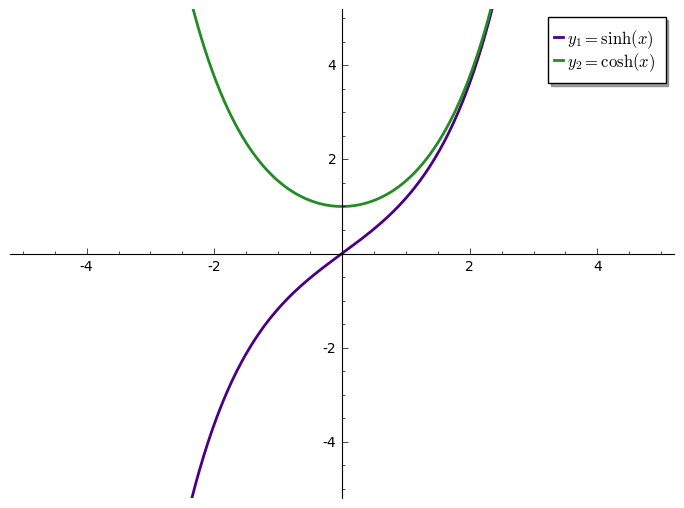
\includegraphics[width=0.6\textwidth]{figs/a.png}
			 	\caption{Hyperbolic Sine and Cosine}
			 	\label{hypGraphs}
			\end{figure} 
		\end{proof}
		% subsection part_b (end)

		\subsection*{Part (c)}
		Use Sage to plot points $(\cosh x, \sinh x)$ for a large range of $x$ values, and see what kind of figure you get. 
		What is it?

		\begin{proof}[Solution]
		Observe Figure \ref{hypPoints} for the requested graph of points of the form $\{ (\cosh x, \sinh x) : x \in(-\pi/2, \pi/2) \}$

			\begin{figure}[h]
				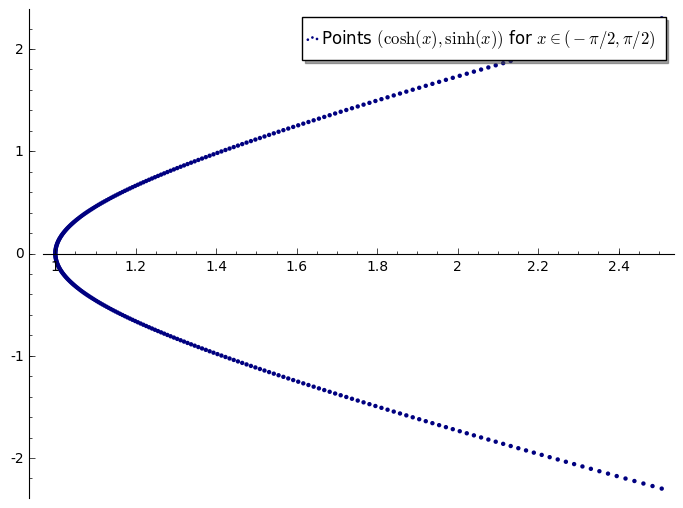
\includegraphics[width=0.6\textwidth]{figs/b.png}
				\caption{Points of the form $(\cosh x, \sinh x)$ for $x \in (-\pi/2, \pi/2)$}
				\label{hypPoints}
			\end{figure}
		\end{proof}
		% subsection part_c (end)
	% section problem_3 (end)
	\pagebreak

	\section*{Problem 4}
	In our discussion of rainbows we had the following picture:
	\begin{figure}[h]
		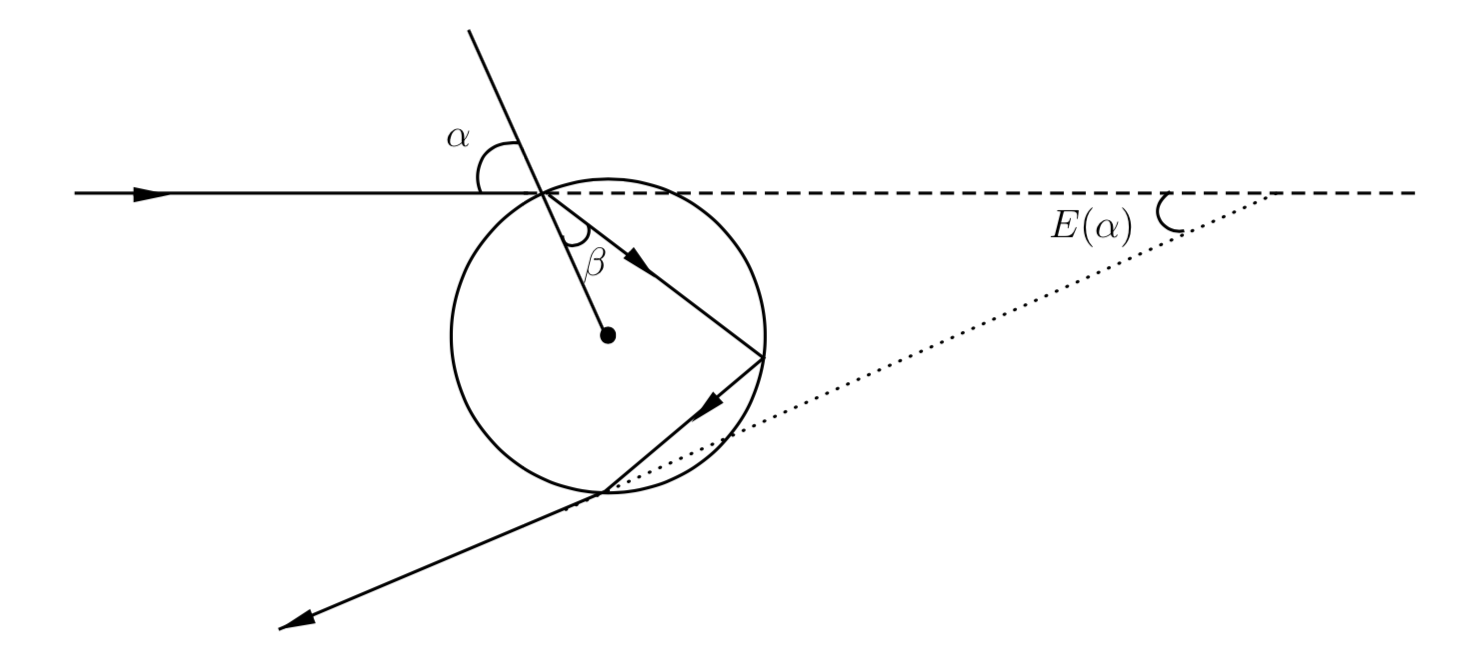
\includegraphics[width=0.8\textwidth]{figs/1.png}
	\end{figure}

		\subsection*{Part (a)}
		Derive the formula $E(\alpha) = 4 \sin^{-1}(\sin \alpha) - 2 \alpha$ where $n$ is the index of refraction for $n$ our light in water. 
		[Hint: If you don’t have notes from class, this is explained in the links I put on the course website.]

		\begin{proof}[Solution]
		From the links on Canvas we have $D_{f}(\alpha) = \pi + 2 \alpha - 4\left( \arcsin \left( \frac{\sin \alpha}{n_{f,w}} \right) \right)$, further, by construction we know that $D_{f}(\alpha)$ and $E(\alpha)$ are supplementary angles, thus we compute:
			\begin{align*}
				E(\alpha) &= \pi - D_{f}(\alpha), \\
				&= \pi - \left[ \pi + 2 \alpha - 4\left( \arcsin \left( \frac{\sin \alpha}{n_{f,w}} \right) \right) \right], \\
				&= -2 \alpha +  4\left( \arcsin \left( \frac{\sin \alpha}{n_{f,w}} \right) \right), \\
				&= 4\left( \arcsin \left( \frac{\sin \alpha}{n_{f,w}} \right) \right) - 2 \alpha.
			\end{align*}
		\end{proof}
		% subsection part_a (end)
		\pagebreak

		\subsection*{Part (b)}
		Use Sage to graph the $E(\alpha)$ function when $n = 1.33$ (red light) and to estimate the maximum value to two decimal places. 
		(One way to do this is to make a rough guess for the maximum value, have Sage graph a horizontal line at that height on the same graph as $E(\alpha)$, and to adjust as necessary). 
		Convert your answer to degrees: this is the angle for the red part of the rainbow.

		\begin{proof}[Solution]
		Observe Figure \ref{redGraph} for the graph of $E(\alpha)$ for red light, and Figure \ref{redMax} for the graph that illustrates the process by which we maximize $E(\alpha)$.
		We estimate that the maximum for $E(\alpha)$ is $42.516^{\circ}$ which is achieved at $\alpha = 59.716^{\circ}$.
			\begin{figure}[h]
				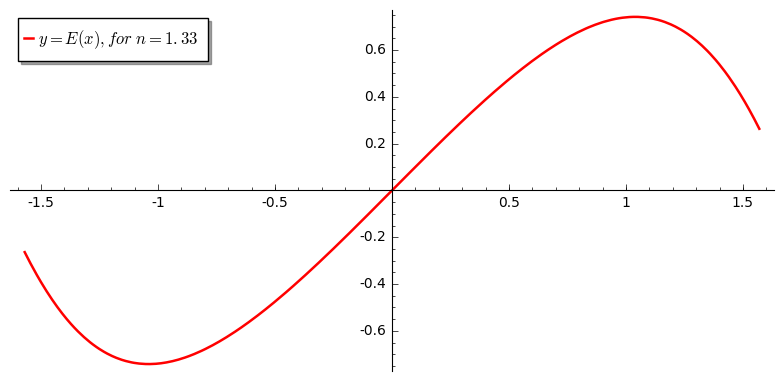
\includegraphics[width=0.6\textwidth]{figs/c.png}
				\caption{$y = E(\alpha)$ for $n = 1.33$}
				\label{redGraph}
			\end{figure}

			\begin{figure}[h]
				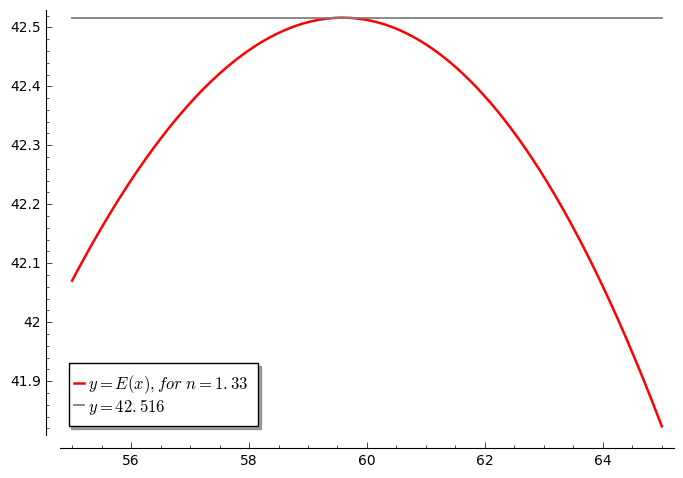
\includegraphics[width=0.8\textwidth]{figs/d.png}
				\caption{Estimating $\max E(\alpha)$}
				\label{redMax}
			\end{figure}
		\end{proof}
		% subsection part_b (end)
		\pagebreak

		\subsection*{Part (c)}
		Use the following indices of refraction for the different colors of light (I left out a couple colors for simplicity):

		\begin{figure}[h]
			\begin{tabular}{c|c|c|c|c}
			& Red & Orange & Green & Blue \\
			\hline
			$n$ & 1.33 & 1.333 & 1.336 & 1.34
			\end{tabular}
			\caption{Refraction Indices}
			\label{refractionIndices}
		\end{figure}
		
		This gives you four functions $E_{R}, E_{O}, E_{G}$, and $E_{B}$ by plugging the different values of $n$ into our $E(\alpha)$ function. 
		Use Sage to plot these four functions on a single graph, and use matching colors (so that $E_{R}$ is shown in red, $E_{O}$ in orange, etc.)

		\begin{proof}[Solution]
		Observe Figure \ref{rainbowGraph} for the graph of $E(\alpha)$ with the various indices of refraction found in Figure \ref{refractionIndices}; for an illustration of how the various maxima of $E(\alpha)$ relate, we have Figure \ref{raibowZoom}.

			\begin{figure}[h]
				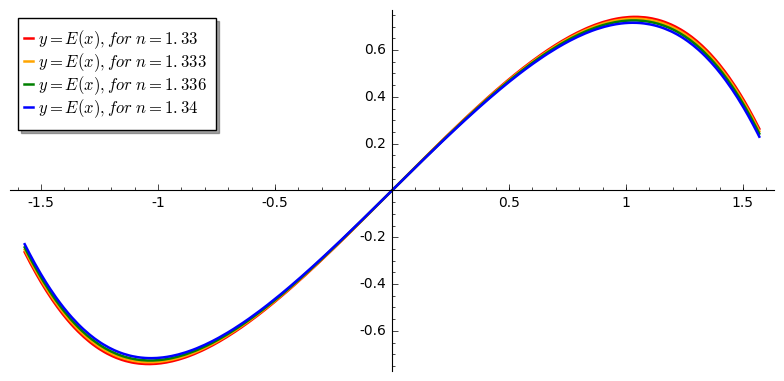
\includegraphics[width=0.6\textwidth]{figs/e.png}
				\caption{$y = E(\alpha)$ for various $n$}
				\label{rainbowGraph}
			\end{figure}

			\begin{figure}[h]
				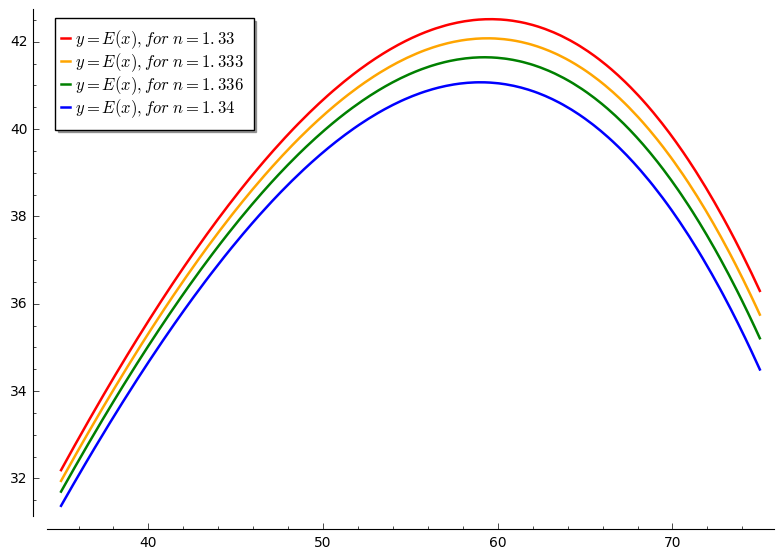
\includegraphics[width=0.6\textwidth]{figs/f.png}
				\caption{Maxima of $E(\alpha)$}
				\label{raibowZoom}
			\end{figure}
		\end{proof}
		% subsection part_c (end)

		\subsection*{Part (d)}
		Give the angles (in degrees) for the orange, green, and blue parts of the rainbow.

		\begin{proof}[Solution]
		Utilizing the same method of estimation as in part b, we have the following maximum angles for $E(\alpha)$ under different values for $n_{f}$; we present them as $(\alpha, E(\alpha))$ ordered pairs:
			\begin{align*}
				\text{Orange} &= (59.48^{\circ}, 42.078^{\circ}) \\
				\text{Green} &= (59.432^{\circ}, 41.643^{\circ}) \\
				\text{Blue} &= (59.153^{\circ}, 41.070^{\circ}).
			\end{align*}
		The Sage-worksheet containing the dirty-work that lead to the above results is attached as Enclosure (1).
		\end{proof}
		% subsection part_d (end)

		\subsection*{Part (e)}
		For red light, there are two incoming angles $\alpha_{1}$ and $\alpha_{2}$ for which the reflected ray has $E = 23^{\circ}$. 
		Find $\alpha_{1}$ and $\alpha_{2}$, giving them in degrees. 
		(You will probably need to use Sage for this part).

		\begin{proof}[Solution]
		As in the previous part, we do the dirty work in Sage (with the worksheet attached) and find that the two incoming angles for which $E(\alpha) = 23^{\circ}$ are $$\alpha_{1} = 23.742^{\circ} \ \text{and} \ \alpha_{2} = 85.627.$$
		\end{proof}
		% subsection part_e (end)
	% section problem_4 (end)
\end{document}